%----------------------------------------------------------------------------------------------------------------------

\begin{frame}{Use of feature information}
\begin{itemize}[noitemsep,label=\textbullet,topsep=2pt,parsep=2pt,partopsep=2pt]
\item Feature based Modeling is a powerful paradigm compared to modeling shapes by mesh or faces.
\item Feature is a geometrical shape characterized by attributes relevant to the domains
\item Part construction is stored as a sequence of features, in form of a Tree.
\item Parametric nature of the Features and Update mechanism, give powerful editing capabilities.
\item Most contemporary CAD packages use this to build and update models.
\end{itemize}
\end{frame}

%----------------------------------------------------------------------------------------------------------------------

\begin{frame}[<+-| alert@+>]{Origination of the Idea}

\begin{itemize}[noitemsep,label=\textbullet,topsep=2pt,parsep=2pt,partopsep=2pt]
\item To concurrently build mid-surfaces as part gets created (called forward create). 
\item At each feature step, shapes are relatively simple than final shape, thus creation of mid-surfaces at each stage is far simpler.

\vspace{0.5cm}

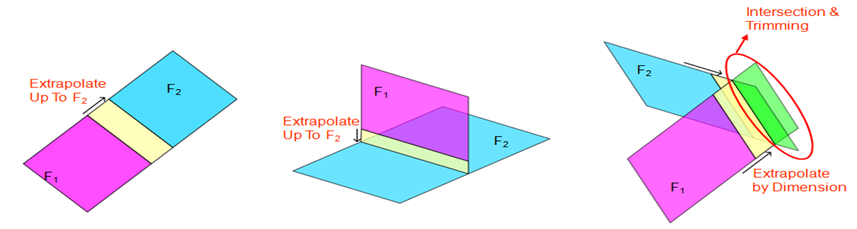
\includegraphics[width=0.95\linewidth]{../Common/images/ExtendTrim.png}

\end{itemize}
\end{frame}


%----------------------------------------------------------------------------------------------------------------------


\begin{frame}[<+-| alert@+>]{Overall Approach}

	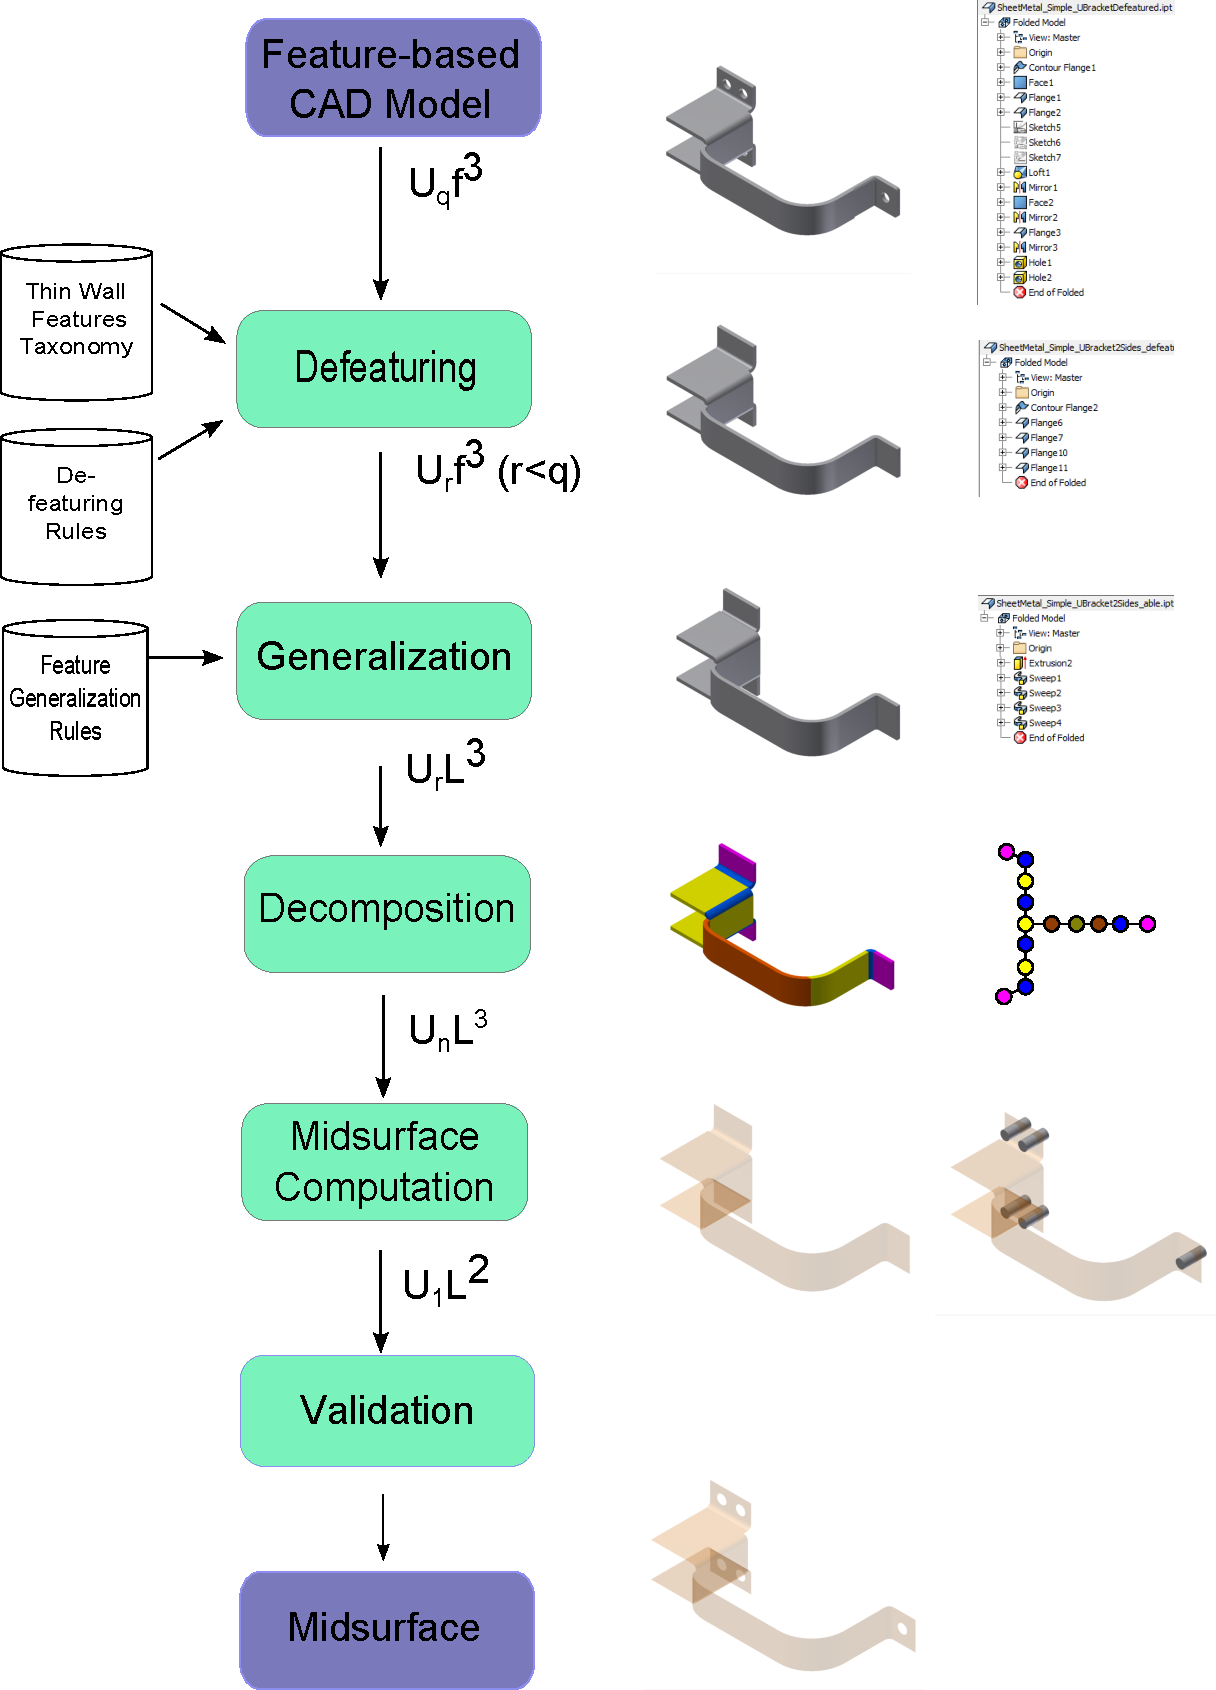
\includegraphics[width=0.5\linewidth]{../Common/images/SystemArchitecture3.pdf}

\end{frame}

%----------------------------------------------------------------------------------------------------------------------


\begin{frame}[<+-| alert@+>]{Overall Approach}

\begin{itemize}[noitemsep,topsep=2pt,parsep=2pt,partopsep=2pt,leftmargin=*]
\item \textbf{Input}: Feature-based CAD models, [Segmentation, decomposition, feature recognition (FR)]

\item \textbf{Defeaturing}:  Computes gross shape by removing irrelevant/superficial features

\item \textbf{Generalization}: Transforms form-features to ``Loft/Sweep'' representations 

\item \textbf{Decomposition}: Cellular decomposition is performed at each Loft/Sweep feature step to form non-volumetrically-overlapping cellular bodies 

\item \textbf{Midsurface Computation}: midsurface-patch generating nodes (solid cells - $sCell$s) and interaction-resolving nodes (interface cells - $iCell$s). 

\item \textbf{Validation}: Topological

\item \textbf{Output}: A well-connected midsurface is then sent to downstream applications such as CAE analysis.
\end{itemize}
\end{frame}


